\documentclass[
	11pt, 
	a4paper, 
	twoside,
	parskip=half*, % Line spacing for paragraphs
	openany, % Chapters can start on any page
	listof=totoc, % Include listings in the table of contents
	bibliography=totoc, % adding a bibliography to the table of contents
	index=totoc, % add index directory to the table of contents
  toc=chapterentrywithdots, % Set dots in the table of contents also for chapters
  numbers=noenddot, % removes the last dot after X.X.X.
  %chapterprefix=true % changes the display of the chapter, adds "Chapter" to the chapter number
]{scrbook}

\usepackage[utf8]{inputenc}
\usepackage{url}
\usepackage[T1]{fontenc}
\usepackage{pdfpages}
\usepackage{textcomp}
\usepackage{amsmath}
\usepackage{svg}

% ---------------------------
% |    Meta-Data for PDF    |
% ---------------------------
\usepackage[
  pdftex,
  pdfauthor={Nathan Rignall},
  pdftitle={Report},
  pdfsubject={600093 - Computational Science},
  pdfproducer={LaTeX},
  pdfcreator={pdfLaTeX},
  pdflang={en},
  bookmarksopen,
  bookmarksnumbered,
]{hyperref}

% ------------------
% |    Settings    |
% ------------------
\usepackage[
    backend=biber, 
    % style=authoryear-icomp, % alphabetic
    % citestyle=authoryear-icomp, % alphabetic, authortitle
    % date=short,
    % backref=true, % Display pages on which the reference is used
    % maxnames=1, % affects the cites
    % maxbibnames=3, % affects the bibliography
    % pagetracker=true,
    % isbn=false,    
    % block=ragged, % break urls
    % firstinits=true, % shorten first names
    % backrefstyle=three+ % Combine pages
    style=authoryear,
    backend=biber,
    urldate=long,
    maxnames=2,
    dashed=false
]{biblatex}

% Distance between bibliographical references
\setlength{\bibitemsep}{.5em}

% Indentation after the first line
\setlength{\bibhang}{2em}

% URL in the bibliography is in angle brackets
\DeclareFieldFormat{url}{<\url{#1}>}

% break too long urls
\setcounter{biburllcpenalty}{7000}
\setcounter{biburlucpenalty}{8000}

% Source of the bibliography file
\bibliography{sources/literature.bib}

% graphics
\usepackage{graphicx}
\graphicspath{ {graphics/} }
\DeclareGraphicsExtensions{.pdf,.png,.jpg,.jpeg,.gif}

% captions
\usepackage{caption}
\usepackage{subcaption}
% % Table layout
\setlength{\tabcolsep}{0.5em} % for the horizontal padding
{\renewcommand{\arraystretch}{1.2} % for the vertical padding

% Table captions
\usepackage{caption} 
\captionsetup[table]{belowskip=12pt,aboveskip=4pt}
\usepackage{diagbox}

% Rotate tables
\usepackage{rotating}
\usepackage{varwidth}

% Footnotes with tables
\usepackage{footnote}
\makesavenoteenv{figure}

% Line breaks in table cells
\newcommand{\specialcell}[2][c]{%
  \begin{tabular}[#1]{@{}c@{}}#2\end{tabular}
}

% rotate content of table cell
\def\rot{\rotatebox} % usage: \rot{angle}{content}
% You can visit this website to find more color codes for LaTeX
% http://latexcolor.com/s

\usepackage{xcolor}

% colors
\definecolor{white}{rgb}{1,1,1}
\definecolor{black}{rgb}{0,0,0}
\definecolor{middlegray}{rgb}{0.5,0.5,0.5}
\definecolor{lightgray}{rgb}{.95,.95,.95}
\definecolor{arsenic}{rgb}{0.23, 0.27, 0.29}
\definecolor{arsenicLight}{rgb}{0.20, 0.20, 0.20}
\definecolor{darkgray}{rgb}{.4,.4,.4}
\definecolor{purple}{rgb}{0.65, 0.12, 0.82}
\definecolor{orange}{rgb}{0.8,0.3,0.3}
\definecolor{yac}{rgb}{0.6,0.6,0.1}
\definecolor{green}{rgb}{.2,0.6,0.3}
\definecolor{azure}{rgb}{0.0, 0.5, 1.0}
\definecolor{editorGray}{rgb}{0.95, 0.95, 0.95}
\definecolor{editorOcher}{rgb}{1, 0.5, 0}
\definecolor{editorGreen}{rgb}{0, 0.5, 0}
\definecolor{orange}{rgb}{1,0.45,0.13}		
\definecolor{olive}{rgb}{0.17,0.59,0.20}
\definecolor{brown}{rgb}{0.69,0.31,0.31}
\definecolor{purple}{rgb}{0.38,0.18,0.81}
\definecolor{lightblue}{rgb}{0.1,0.57,0.7}
\definecolor{lightred}{rgb}{1,0.4,0.5}

\definecolor{vscodered}{HTML}{E53935}
\definecolor{vscodelightred}{HTML}{EF5350}
\definecolor{vscodeblue}{HTML}{1565C0}
\definecolor{vscodegreen}{HTML}{66BB6A}

\definecolor{lightblack}{HTML}{212121}
\definecolor{darkraspberry}{rgb}{0.53, 0.15, 0.34}

% blue hues
\definecolor{bleudefrance}{rgb}{0.19, 0.55, 0.91}
\definecolor{brandeisblue}{rgb}{0.0, 0.44, 1.0}
\definecolor{blue(ncs)}{rgb}{0.0, 0.53, 0.74}
\definecolor{coolblack}{rgb}{0.0, 0.18, 0.39}

% red hues
\definecolor{coralred}{rgb}{1.0, 0.25, 0.25}
\definecolor{darkred}{rgb}{0.55, 0.0, 0.0}

% geometry
\usepackage{geometry}
\geometry{left=25mm, right=25mm, top=25mm, bottom=30mm}

\usepackage[automark]{scrlayer-scrpage}
\pagestyle{scrheadings}
\automark*[section]{}
\ohead{\headmark} % name of the current section
\ihead{}
\ofoot{\thepage} % page number

% footnote gap
\addtolength{\skip\footins}{1ex}
\addtolength{\footnotesep}{0.5ex}

% prevent footnote page break
\interfootnotelinepenalty=10000

% prevent page break in the middle of a paragraph
\widowpenalties 1 10000

% line spacing
\usepackage[onehalfspacing]{setspace}

% text does not have to go to the end of a page
\raggedbottom

% space before and after chapter headings
\RedeclareSectionCommand[beforeskip=0pt,afterskip=.6cm,font=\fontsize{18}{20}\selectfont]{chapter}
% \RedeclareSectionCommand[beforeskip=10pt,afterskip=.3cm,font=\fontsize{18}{25}\selectfont]{section}
% \RedeclareSectionCommand[beforeskip=10pt,afterskip=.3cm,font=\fontsize{16}{25}\selectfont]{subsection}
% \RedeclareSectionCommand[beforeskip=0pt,afterskip=.3cm,font=\fontsize{14}{25}\selectfont]{subsubsection}

\usepackage{mwe}

% chapter style
\renewcommand*{\chapterformat}{%
  \thechapter\enskip
  \textcolor{gray!70}{\rule[-\dp\strutbox]{1pt}{\baselineskip}}\enskip
}
\setkomafont{disposition}{\normalcolor\bfseries}

% adjust paragraphs
%\addtokomafont{paragraph}{\itshape}
%\setkomafont{subsubsection}{\large}
%\setkomafont{paragraph}{\normalsize\itshape}
\setkomafont{paragraph}{\normalsize}

% % layout of the paragraphs
% % paragraphs look like the subsubsections
% \RedeclareSectionCommands[
%     beforeskip=-3.25ex plus -1ex minus -0.2ex,
%     afterskip=1sp, % smallest possible positive value
% ]{paragraph,subparagraph}

% Bold caption labels
\setkomafont{captionlabel}{\normalsize\bfseries} 
% \usepackage[font=sf]{caption} % Captions without serifs
% for the links in toc
\usepackage{hyperref}
\hypersetup{
    colorlinks,
    citecolor=black,
    filecolor=black,
    linkcolor=black,
    urlcolor=black,
    pdfstartview= % fit zoom size to the viewer
}
%\newcommand{\code}[1]{\colorbox{lightgray}{\texttt{#1}}}
%\lstinline{snippet}
%http://tex.stackexchange.com/questions/65291/code-snippet-in-text

% This "\code{my code}" can be used to highlight small code snippets in the text like names of variables or methods.
\newcommand{\code}[1]{\textcolor{black}{\texttt{#1}}}

% The "\todo{this still has to be done}" is a command that highlights todos in the text.
\newcommand{\todo}[1]{\textcolor{vscodered}{TODO: \texttt{#1}}}
% Adding package bookmark improves bookmarks handling.
% More features and faster updated bookmarks.
\usepackage{bookmark}

% \pdfbookmark[<level>]{<title>}{<dest>}

% toc is part of the bookmarks but not part the toc itself
% \pdfbookmark[section]{\contentsname}{toc}


\begin{document}

% -------------------
% |    Titlepage    |
% -------------------
\titlehead{\centering University of Hull}
\subject{600093 - Computational Science}
\title{Cellular Automata}
\author{Nathan Rignall}
\immediate\write18{./wordcount.sh > wordcount.aux }
\date{\today\\ Word count: \input{wordcount.aux}}
\maketitle

% ---------------------------
% |    Table of contents    |
% ---------------------------
\pdfbookmark[section]{\contentsname}{toc}
\newpage\thispagestyle{empty}
{
  \pagestyle{empty}
  \addtocontents{toc}{\protect\thispagestyle{empty}} 
  \tableofcontents
  \clearpage
}

% ------------------
% |    Chapters    |
% ------------------
\mainmatter
\setcounter{page}{1}
\chapter{Introduction}

This report shall show the steps taken to simulate the growth of cancer cells in a tissue using the Gompertz Equation to model growth.

Growth for individual cells can be modelled using a differential equation so that the number of cells is a function of time, shown in Equation \ref{eq:1}.
The Gompertz Model of Cell Growth works well in this application because it can accurately model the non exponential nature of cell growth \autocite{tatroMathematicsCancerFitting2018}.
Once an area has reached it's capacity no more tumour cells can form, hence the cells must begin to move through a tissue.
This movement can be simulated using simple random walk algorithms \autocite{codlingRandomWalkModels2008}.

\begin{equation}
    \frac{dN}{dt} = kNln\left(\frac{M}{N} \right) \label{eq:1}
\end{equation}

This paper specifically shall analyse the computational complexity of such models and evaluate the differences between simulation techniques.
The underlying implementation shall be investigated, including random algorithms and accuracy of simulations on computer systems.

Simulations shall use Rust as the programming language, for its performance properties as a low level language \autocite{adamRustConciseOverview2023}.
It also allows for fine control over types, which can be useful for numerical simulations.
Fine-grained benchmarks shall be used to evaluate the performance of the simulations using the criterion library \autocite{heislerBheislerCriterionRs2024}.
Analysis of data generated shall be done using Python with Matplotlib and Numpy.
\chapter{Methodology}

- Does the growth reach a steady state? (at t=1200)
- Will the rate of growth reach a steady state or will the number increase as you keep increasing the size of the grid?
- What will happen if the value of M is changed - pick two values on either side of the value given.
- Comment on computational complexity of each method. (note you had been asked to locate common-points which both methods reach)

\section{Cell Movement}

5 marks for definitions of distributions and reasons behind the choice of distribution

The random movement of cells should be modelled using a probability distribution


There are several probability distributions that can be classified as discrete or continuous, we will analyse uniform, bernoulli and beta.

The uniform distribution is usually regarded as a continuous distribution but can also be used to model discrete variables. 

Area under the graph is one

\[ f(x) =\begin{cases}a & \text{if } x = 1\\b & \text{if } x = 0\end{cases}\]

\[ f(x) =\begin{cases}1 & \text{for } 0  \leq x  \leq  1\\0 & \text{otherwise}\end{cases}\]

Uniform distribution
Definition of distributions
Uniform distributions
Bernoulli Distribution

Bias introduced with different distributions


When all directions are equally probable a uniform distribution could be used.

If a Bernoulli distribution was selected, it would introduce a bias to the direction of movement
This could be desired in a complex model where factors such as surface tension affect the direction of movement


% how random numbers are actually generated in rust



% complexity of the different movements
%  all o^n but increase the multiplier of n







Movement directions

'Complexity of direction methods'

\clearpage

\begin{figure}[ht]
    \centering
    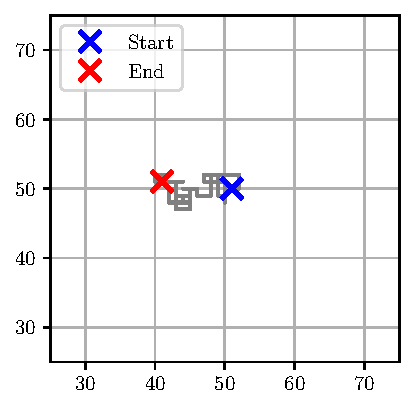
\includegraphics[width=5cm]{task1-1}
    \caption[Square cell movement plot]{Square cell movement plot}
    \label{fig:task1-1}
\end{figure}

\begin{figure}[ht]
    \centering
    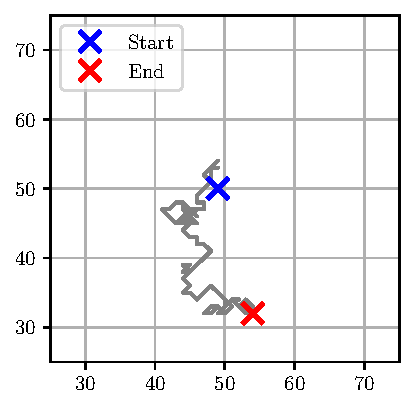
\includegraphics[width=5cm]{task1-2}
    \caption[Diagonal cell movement plot]{Diagonal cell movement plot}
    \label{fig:task1-2}
\end{figure}

\begin{figure}[ht]
    \centering
    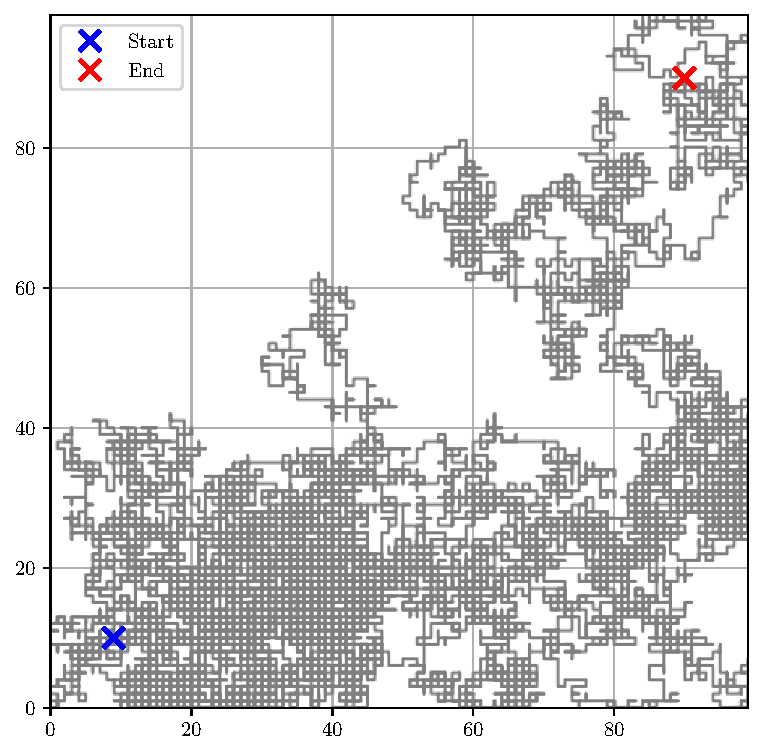
\includegraphics[width=10cm]{task1-1-fill}
    \caption[Square cell movement plot with fill]{Square cell movement plot with fill}
    \label{fig:task1-1-fill}
\end{figure}

\begin{figure}[ht]
    \centering
    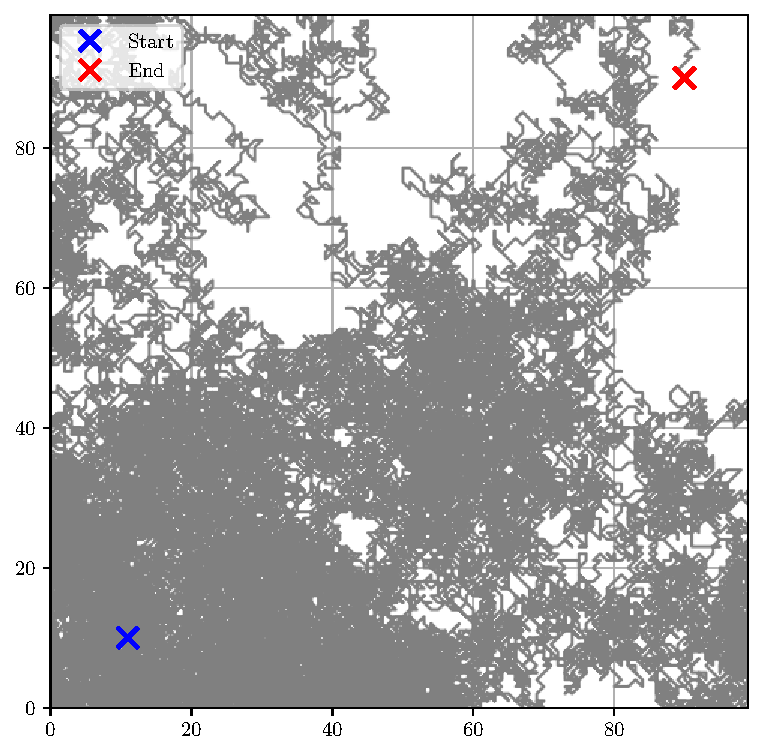
\includegraphics[width=10cm]{task1-2-fill}
    \caption[Diagonal cell movement plot with fill]{Diagonal cell movement plot with fill}
    \label{fig:task1-2-fill}
\end{figure}

\clearpage

\begin{figure}[ht]
    \centering
    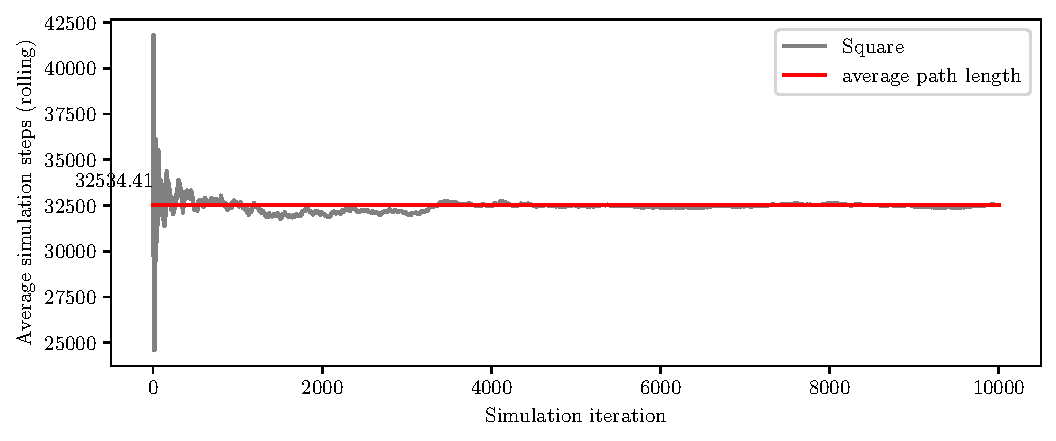
\includegraphics[width=14cm]{task1-compare-square-roll}
    \caption[Square cell simulation steps]{Square cell simulation steps}
    \label{fig:task1-compare-square-roll}
\end{figure}

\begin{figure}[ht]
    \centering
    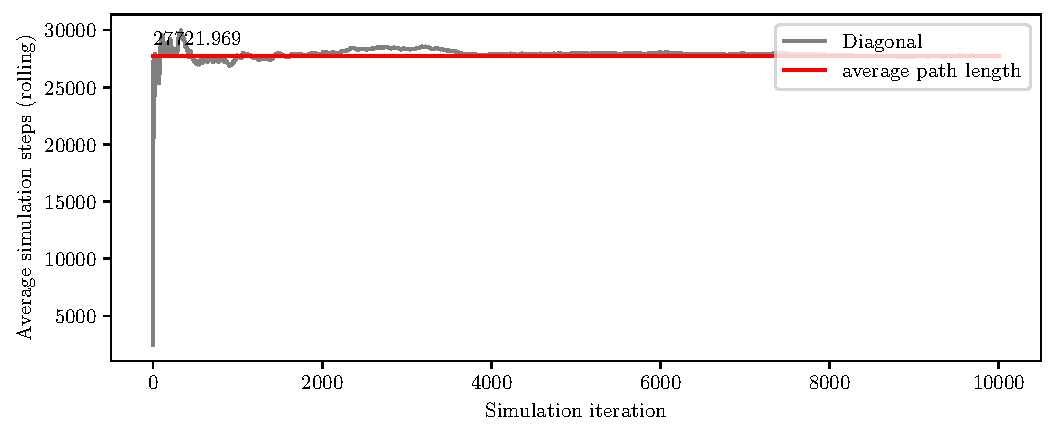
\includegraphics[width=14cm]{task1-compare-diagonal-roll}
    \caption[Diagonal cell simulation steps]{Diagonal cell simulation steps}
    \label{fig:task1-compare-diagonal-roll}
\end{figure}

\clearpage

Non Diagonal - (74, 67) - (55, 40) - 32534.4086
Diagonal - (74, 67) - (55, 40) - 23247.6747

\begin{figure}[ht]
    \centering
    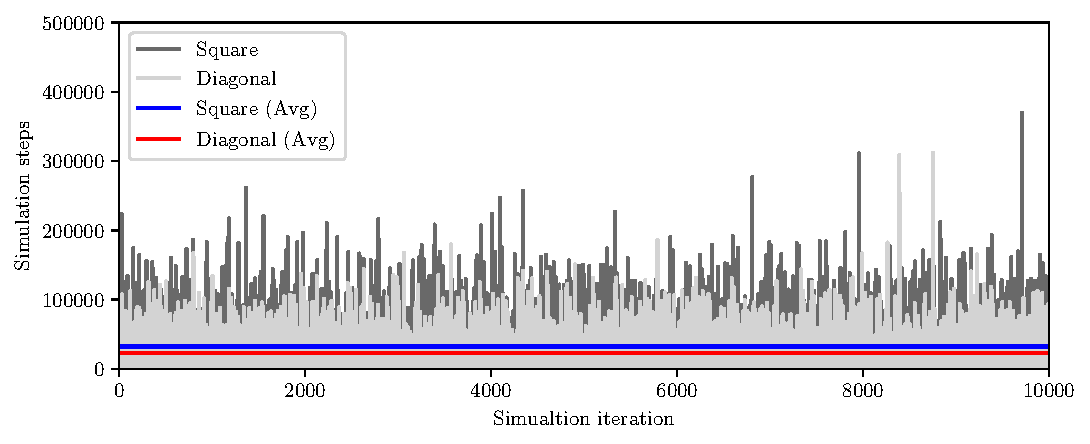
\includegraphics[width=14cm]{task1-compare-single}
    \caption[Comparison of square and diagonal simulation steps]{Comparison of square and diagonal simulation steps}
    \label{fig:task1-compare-single}
\end{figure}

\begin{figure}[ht]
    \centering
    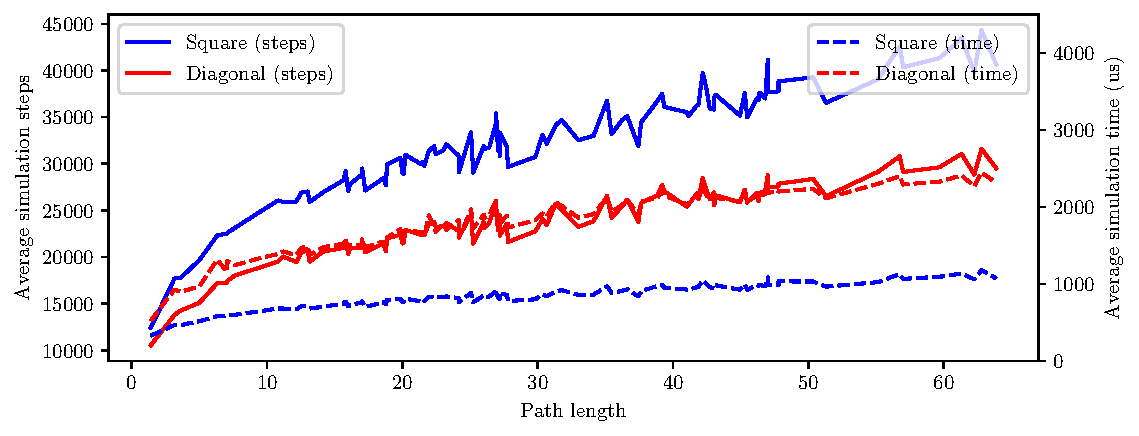
\includegraphics[width=14cm]{task1-compare}
    \caption[Comparison of multiple square and diagonal simulation steps]{Comparison of multiple square and diagonal simulation steps}
    \label{fig:task1-compare}
\end{figure}

\clearpage

Average steps factor: 0.7393451245144123
Average time factor: 2.143568060901476

\begin{figure}[ht]
    \centering
    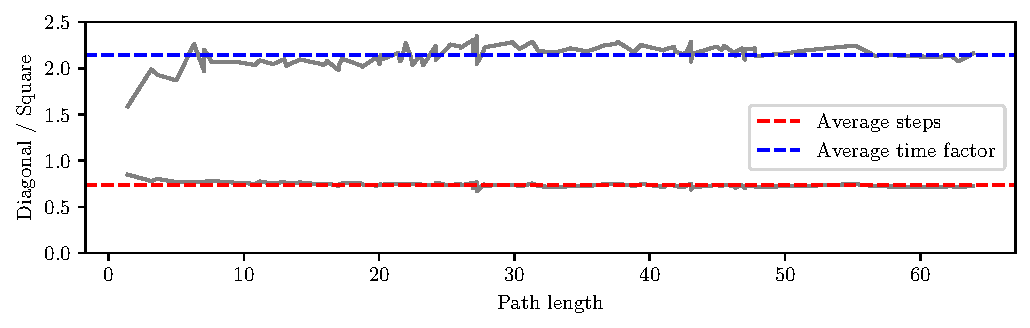
\includegraphics[width=14cm]{task1-factor-length}
    \caption[Comparison of multiple square and diagonal simulation steps (factor length)]{Comparison of multiple square and diagonal simulation steps (factor length)}
    \label{fig:task1-factor-length}
\end{figure}

\clearpage

\begin{figure}[ht]
    \centering
    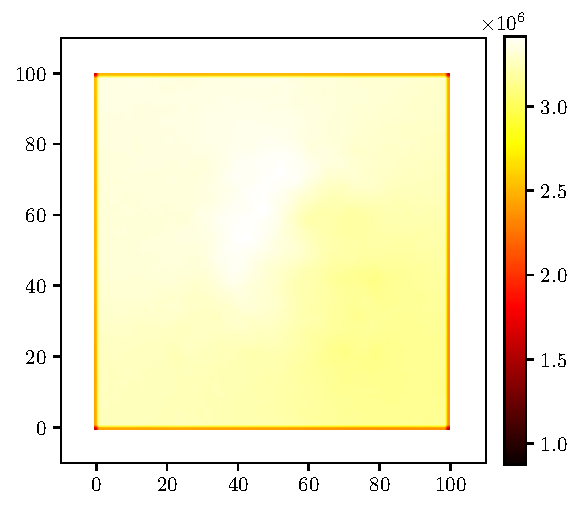
\includegraphics[width=7cm]{task1-visited-square}
    \caption[Visited cells in square simulation heatmap]{Visited cells in square simulation heatmap}
    \label{fig:task1-visited-square}
\end{figure}

\begin{figure}[ht]
    \centering
    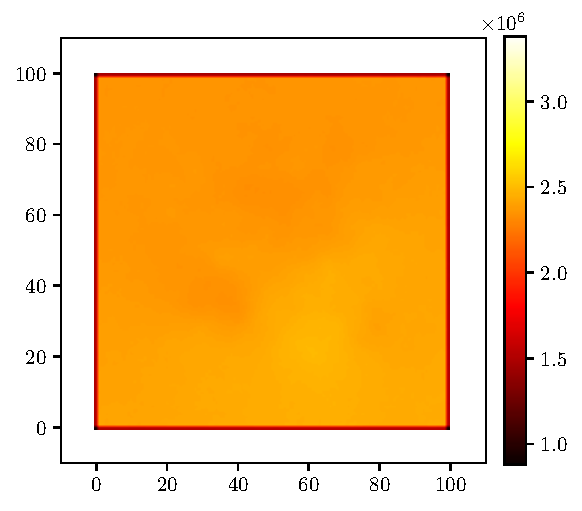
\includegraphics[width=7cm]{task1-visited-diagonal}
    \caption[Visited cells in diagonal simulation heatmap]{Visited cells in diagonal simulation heatmap}
    \label{fig:task1-visited-diagonal}
\end{figure}

\begin{figure}[ht]
    \centering
    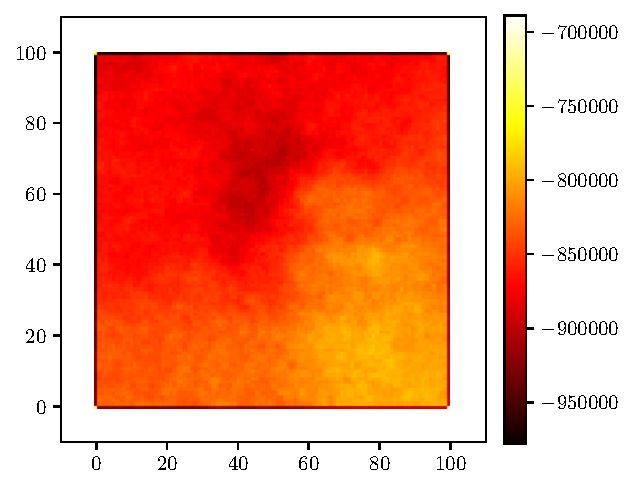
\includegraphics[width=7cm]{task1-visited-diff}
    \caption[Difference in visited cells between square and diagonal simulation heatmap]{Difference in visited cells between square and diagonal simulation heatmap}
    \label{fig:task1-visited-diff}
\end{figure}

\clearpage

\section{Cell Growth}
10 marks for basic simulation, 5 marks for showing time to reach final time 
You can also use analytical methods to do the same

5 marks for the part where you suggest what happens when the value of M changes, and why this is important
\[ \frac{dN}{dt}  = kNln\left(\frac{M}{n} \right) \]

\clearpage

\begin{figure}[ht]
    \centering
    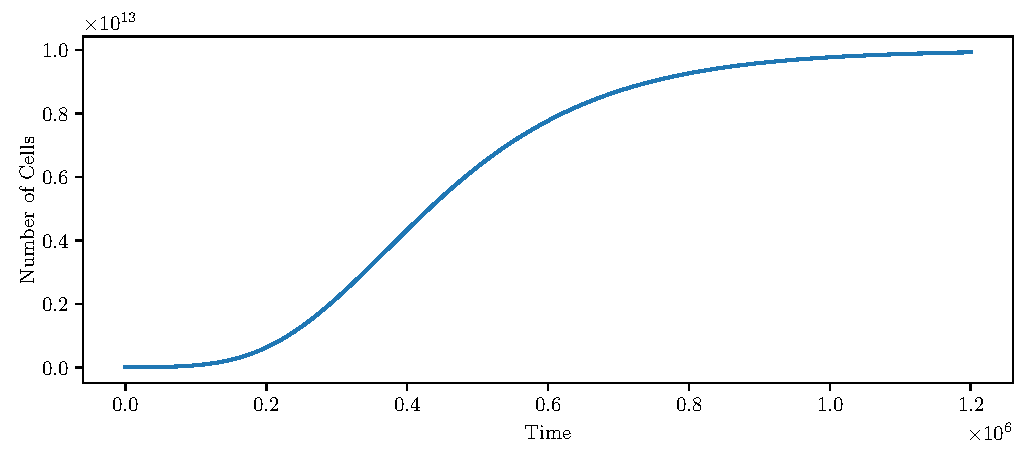
\includegraphics[width=14cm]{task2-1}
    \caption[Cell growth simulation]{Cell growth simulation}
    \label{fig:task2-1}
\end{figure}

\begin{figure}[ht]
    \centering
    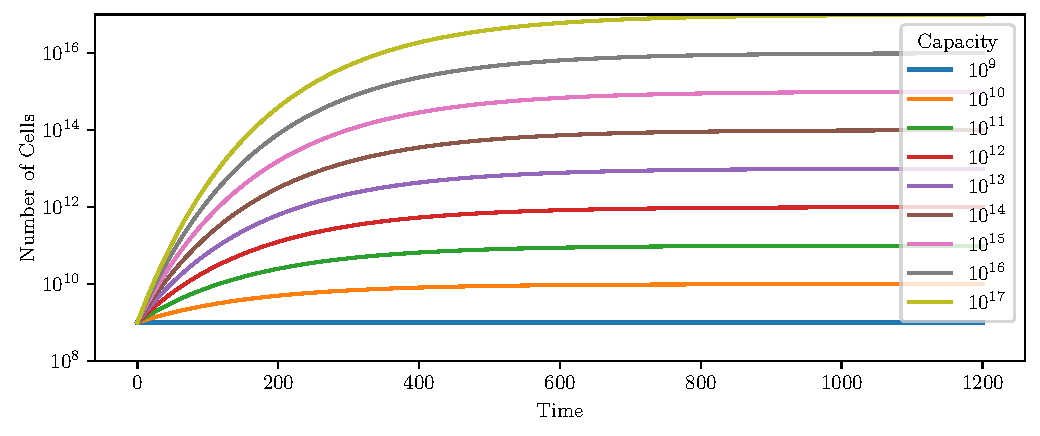
\includegraphics[width=14cm]{task2-1-m}
    \caption[Cell growth simulation with different capacity values]{Cell growth simulation with different capacity values}
    \label{fig:task2-1-m}
\end{figure}

\clearpage

\begin{figure}[ht]
    \centering
    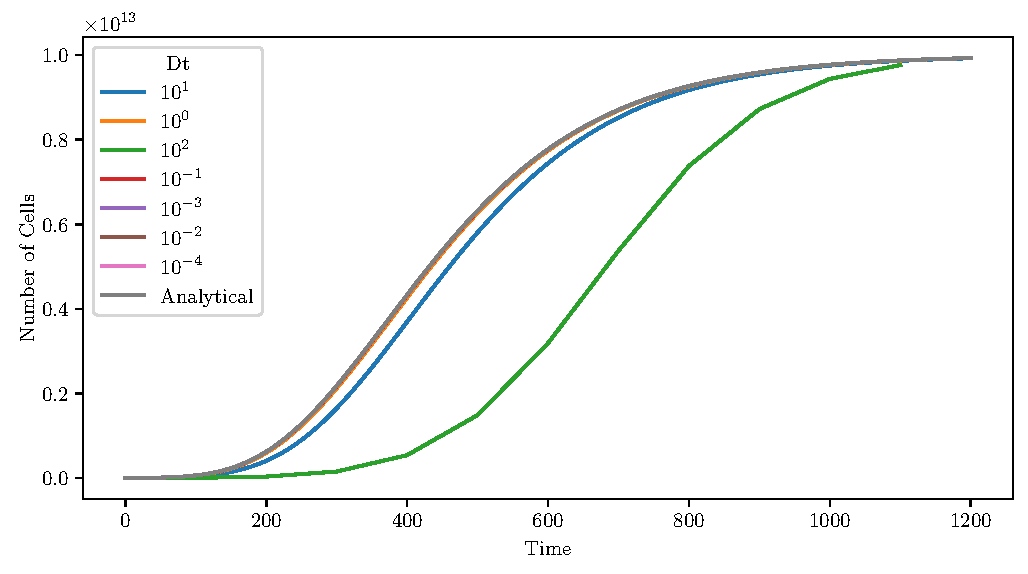
\includegraphics[width=14cm]{task2-1-h}
    \caption[Cell growth simulation with different dt values]{Cell growth simulation with different dt values}
    \label{fig:task2-1-h}
\end{figure}

\begin{figure}[ht]
    \centering
    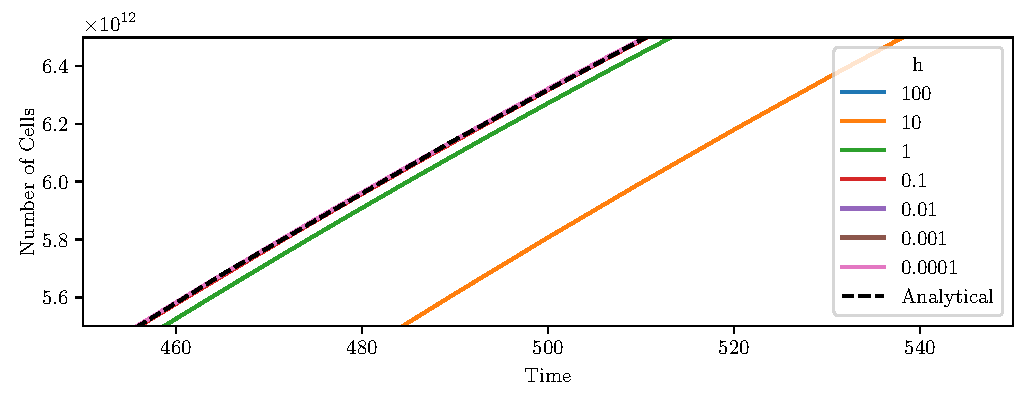
\includegraphics[width=14cm]{task2-1-h-zoom}
    \caption[Cell growth simulation with different dt values (zoomed)]{Cell growth simulation with different dt values (zoomed)}
    \label{fig:task2-1-h-zoom}
\end{figure}

\begin{center}
\begin{tabular}{c | c} 
    h & Error \\
    \hline
    100 & 66.69\% \\
    10 & 5.296\% \\
    1 & 0.5238\% \\
    0.1 & 0.05233\% \\
    0.01 & 0.005233\% \\
    0.001 & 0.0005239\% \\
    0.0001 & 5.82e-05\% \\
    Analytical & 0.0 \\
\end{tabular}
\end{center}

\clearpage

\begin{figure}[ht]
    \centering
    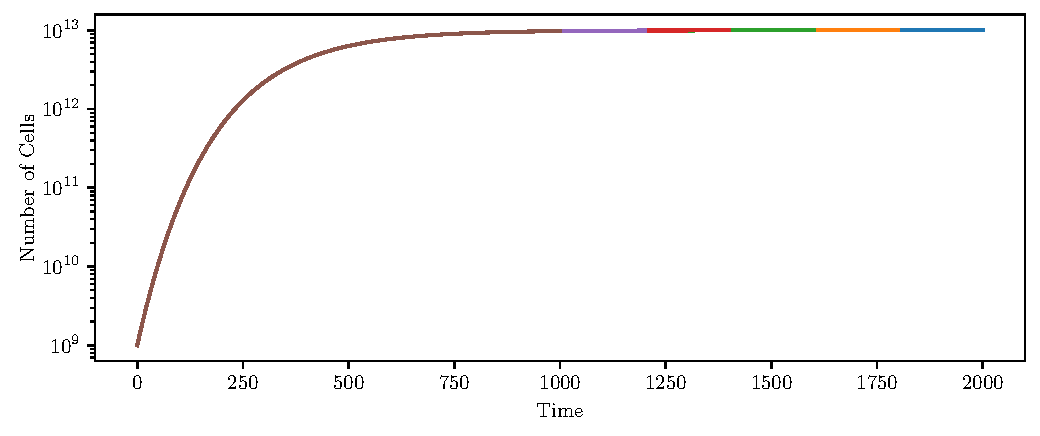
\includegraphics[width=14cm]{task2-1-t}
    \caption[Cell growth simulation with different T values]{Cell growth simulation with different T values}
    \label{fig:task2-1-t}
\end{figure}

\begin{center}
\begin{tabular}{c | c c} 
    T & Cells & \ Full \\
    \hline
    2000 & 1.00e+13 & 0.9999\% \\
    1800 & 1.00e+13 & 0.9998\% \\
    1600 & 9.99e+12 & 0.9994\% \\
    1400 & 9.98e+12 & 0.9979\% \\
    1200 & 9.93e+12 & 0.9931\% \\
    1000 & 9.77e+12 & 0.9774\% \\    
\end{tabular}
\end{center}

\clearpage

\begin{figure}[ht]
    \centering
    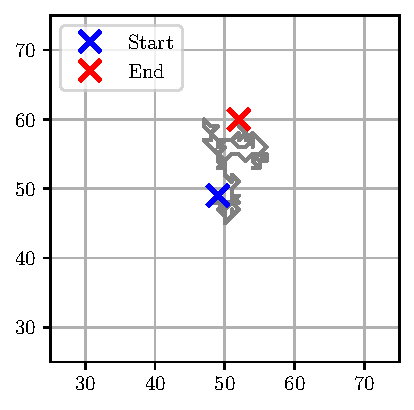
\includegraphics[width=5cm]{task2-2}
    \caption[Cell growth simulation with diagonal movement]{Cell growth simulation with diagonal movement}
    \label{fig:task2-2}
\end{figure}

\clearpage

\begin{figure}[ht]
    \centering
    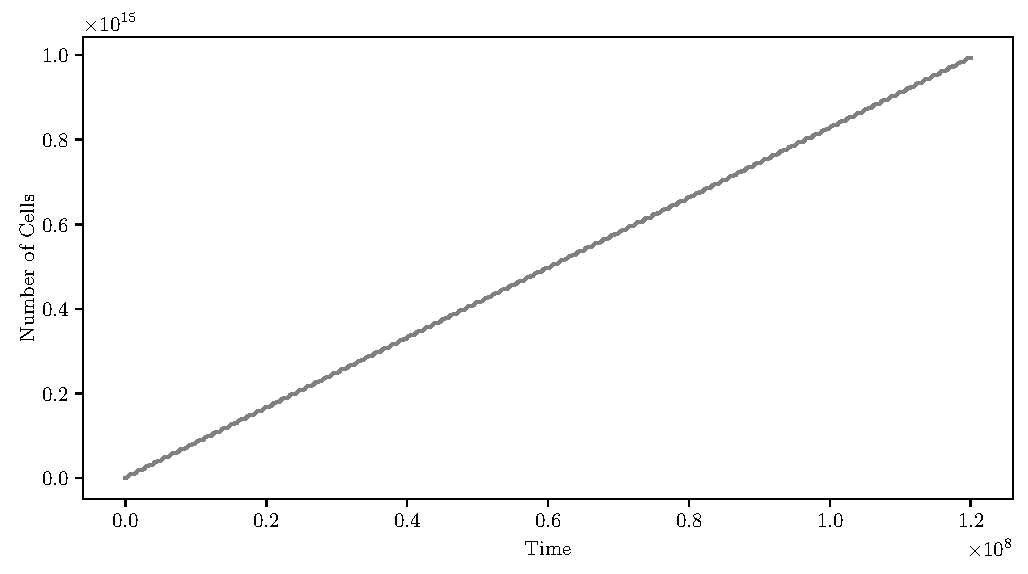
\includegraphics[width=14cm]{task2-2-total}
    \caption[Cell growth simulation with diagonal movement (total cells)]{Cell growth simulation with diagonal movement (total cells)}
    \label{fig:task2-2-total}
\end{figure}

\begin{figure}[ht]
    \centering
    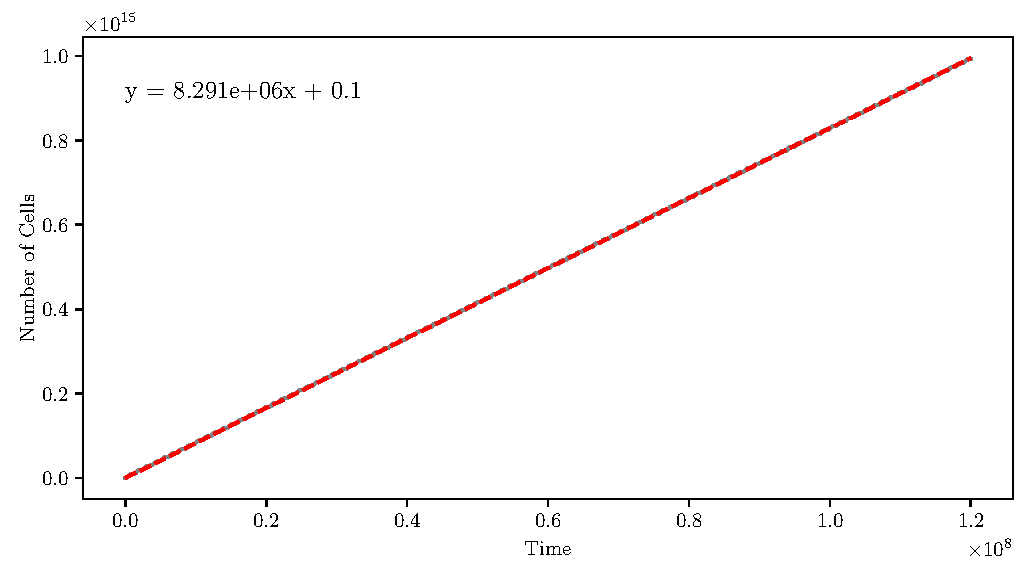
\includegraphics[width=14cm]{task2-2-total-linear}
    \caption[Cell growth simulation with diagonal movement (total cells) linear estimation]{Cell growth simulation with diagonal movement (total cells) linear estimation}
    \label{fig:task2-2-total-linear}
\end{figure}

\chapter{Conclusion}

This report successfully implemented a simulation of the growth of cancer cells in a tissue using computational techniques.
The model's complexity is of $\bigO(n) + \bigO(n) = \bigO(n)$, where $n$ is the number of steps in the simulation.

% The euler method was used 

Currently the model has no interaction between movement and growth.
A Bernoulli distribution for movement based on surface tension and leaky boundary conditions could be implemented to simulate the growth of cancer cells more accurately.

% Also talk about edge processing and limited requirements
% Issues with the numerical strategy include the accuracy of the simulation and the computation time.

% -----------------
% |    Indexes    |
% -----------------
\listoffigures
\listoftables

% ----------------------
% |    Bibliography    |
% ----------------------
\printbibliography

% --------------------
% |    Appendices    |
% --------------------
\appendix
\chapter{Appendix}

Integration using substitution

\begin{eqnarray*}
\frac{dN}{dt}                                &=& kNln\left(\frac{M}{N} \right) \\
\frac{dN}{Nln\left(\frac{M}{N} \right)}      &=& kdt \\
\int \frac{dN}{Nln\left(\frac{M}{N} \right)} &=& \int kdt \\
\end{eqnarray*}

\begin{align*}
\text{with}\ u &= ln\left(\frac{M}{N} \right) & \text{and}\ && \frac{du}{dN} &= -\frac{1}{N}
\end{align*}
% dN = -Ndu \]

\begin{eqnarray*}
\int \frac{-Ndu}{Nu} &=& \int kdt \\
\int -\frac{1}{u}du &=& \int kdt \\
-ln\left(|{u}| \right) &=& kt + c \\
ln\left(|{u}| \right) &=& -kt - c \\
ln\left(\left|\ln\left(\dfrac{M}{N}\right)\right|\right) &=& -kt - c \\
ln\left(\dfrac{M}{N}\right) &=& e^{-kt - c} \\
\dfrac{M}{N}                &=& e^{e^{-kt - c}} \\
N                           &=& \dfrac{M}{e^{e^{-kt - c}}}
\end{eqnarray*}

\clearpage

Calculate c using the initial values

\begin{align*}
    M &= 10^{13} & k &= 0.06 & N &= 10^9 & t &= 0
\end{align*}

\begin{eqnarray*}
10^9        &=& \dfrac{10^{13}}{e^{e^{-0.006(0) - c}}} \\
e^{e^{-c}}  &=& \dfrac{10^{13}}{10^9} \\
e^{e^{-c}}  &=& {10^4} \\
-c          &=& ln\left(\left|\ln\left({10^4}\right)\right|\right) \\
c           &=& -ln\left(\left|\ln\left({10^4}\right)\right|\right) \\
\end{eqnarray*}

Substitute c back in and simplify

\begin{eqnarray*}
N &=& \dfrac{M}{e^{e^{-kt + ln\left(\left|\ln\left({10^4}\right)\right|\right)}}} \\
  &=& \dfrac{M}{e^{e^{-kt} e^{ln\left(\left|\ln\left({10^4}\right)\right|\right)}}} \\
  &=& \dfrac{M}{e^{e^{-kt} \ln\left({10^4}\right)}} \\
  &=& \dfrac{M}{(e^{\ln\left({10^4}\right)})^{e^{-kt}}} \\
N  &=& \dfrac{M}{10^{4e^{-kt}}}
\end{eqnarray*}

\clearpage

\end{document}
